\section{Overview}
Bluetooth devices operate in the ISM 2.4 Ghz band, a portion of the spectrum that can be utilized without licenses.
The spectrum, from 2400 to 2483.5 MHz, is partitioned in 79 radio channels.
The radio channels start at 2402 MHz and are 1 MHz wide.
Given that the ISM spectrum is utilized by many other technologies such as 802.11g/n, cordless phones and microwave ovens, Bluetooth has been designed to be noise tolerant. 
To achieve noise tolerance Bluetooth devices switch between the 79 available channels 1600 times per second in a pseudo-random fashion. This technique is called \emph{Channel Hopping}.
Two or more devices that have the same hopping pattern share a physical channel and are considered part of the same piconet.

\subsection{Piconets}
Piconets are the most basic form of Bluetooth communication upon which all other protocols are layered on.
In a piconet a device must act as a master and all the other devices as slaves.
The physical channel is divided into slots numbered according to the Bluetooth clock of the master.
A time division duplex scheme is used to schedule access to the channel and allow master and slaves to communicate.
All the communication in a piconet is between master and slaves, there is never direct communication between slaves.

\paragraph{Addressing}
Bluetooth radios, not unlike other network cards, are supplied by the manufacturer with a 48 bit long mac address.
This address is used to determine the hopping pattern of a device and to distinguish devices during the inquiry scan phase.
Devices participating in a piconet are addressed with a 3 bit long identifier which is only valid until they are active.
This means that only 7 slaves can concurrently participate in a piconet.
The master can keep track of inactive (parked) members of a piconet using a 8 bit long identifier.

\paragraph{Scatternets}
A device may be part of more than one piconet at the same time, but can only be the master of one. This kind of set-up is called a scatternet.
At a physical level this is achieved by time-sharing access to the Bluetooth radio.

\begin{figure}[h!]
  \centering
  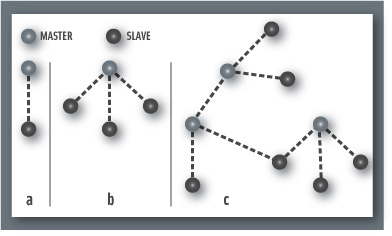
\includegraphics[width=0.7\textwidth]{img/piconets.jpg} 
  \caption{Piconets with a single slave operation (a), a multi-slave operation (b) and a scatternet operation (c).}
\end{figure}

\paragraph{Adaptive Frequency Hopping}
In a piconet the master may decide to alter the hopping sequence to only use a subset of the available 79 channels. The master will exclude  noisy channels and then communicate the new hopping pattern to all the slaves.

\subsection{Connection setup}
A connection is normally created following two steps: inquiry and page.
The inquiry scan is necessary to discover the mac addresses of devices that are in range and the paging procedure is used to establish the actual connection.
In the inquiry phase the source sends out inqury packets and then listens for inquiry reply.
If a listening device is in the inquiry phase it can receive and reply to such packets.
After the inquiry scan is complete a paging procedure can be started to establish the connection.
The device which starts the paging procedure will become master of the piconet formed as a result.

\subsection{Range}
Bluetooth divides devices into three classes based on how much transmission power they have, the transmission power influences the distance 

\vspace{0.3cm}
\begin{tabular}{|c|r|r|}
 \hline
 class & transmission power output & range \\ \hline
 1 & 100 mW & 100 meters \\
 2 & 2.5 mW & 10 meters \\
 3 & 1 mW & 1 meter \\
 \hline
\end{tabular}
\vspace{0.3cm} 

\noindent
Most modern smartphones are class 2 devices

\subsection{Baseband}
The \emph{baseband} implements the medium access control and physical layer parts of the Bluetooth system.
It manages physical channels and links, hop selection and scanning for nearby devices (inquiry scan).

